\documentclass[a4paper]{jpconf}
\usepackage{graphicx}
\begin{document}
\title{The CMS Data Aggregation System}

\author{Valentin Kuznetsov}
\address{Cornell University, Ithaca, New York, USA}
\ead{vkuznet@gmail.com}

\author{Dave Evans}
\address{Fermilab, Batavia, Illinois, USA}
\ead{evansde@fnal.gov}

\author{Simon Matson}
\address{Bristol University, Bristol, UK}
\ead{s.metson@bristol.ac.uk}


%In a large modern enterprise, information is almost inevitably distributed among several database management systems. Despite considerable attention from the research community, relatively few commercial systems have attempted to address this issue. This article describes the technology that enables clients of IBM's federated database engine to access and integrate the data and specialized computational capabilities of a wide range of relational and non­relational data sources.

\begin{abstract}
A metadata plays significant role in a large modern enterprises, research experiments,
digital libraries where it comes from different sources and distributed in a 
variety of forms and digital formats. It is organized and managed by constantly
evolving software using both relational and nonrelational data sources. There is
a big demand to access information from multiple sources.
Here we discuss a new data aggregation system which deliver and cache information 
from different relational and nonrelational data sources on a concrete example 
of large scale High-Energy physics experiment.
\end{abstract}

\newpage

\section{Introduction}
The CERN, the European Organization for Nuclear Research, plays a leading
role in fundamental studies of physics. But apart from scientific community 
it is known as a place where World Wide Web was born. At that time the 
information look-up among hyperlinks represents a certain challenge for scientists.
Today, the Large Hadron Collider (LHC) at CERN is marking a new era of High Energy
Physics (HEP), promising to deliver a few PB of data each year. Scientists are
facing another set of problems from distributed computing to multi-dimentional
view on information retrieval. One of the aspect of such research is an efficient
and at the same time precise look-up of produced meta-data, which comes in variety 
of forms and digital formats. As was pointed out in \cite{Amr} a mixed content and 
mixed metadata and metadata consistency should be considered as a whole in design 
of the system to successful information discovery. 

The CMS, the Compact Muon Solenoid experiment, operated at LHC,
represents an heterogeneous environment of distributing computing, relational and
nonrelational data sources where we face this problem. The computing resources
are distributed among almost 40 countries, 183 institutions and more then 3000 physicists.
Broad variety of RDMS systems at different data centers collect a various
metadata information, including data location and transfer, detector conditions,
calibrations constants, simulation information, etc. Moreover the development
of those components were done in parallel by different group and technology
tools. Therefore a wide spectrum of data services and
data formats represents a problem of information discovery.

\section{Related Work}
Even though the idea of querying relation databases via keyword based search
algorithm is not knew it is still under significant activity in computer
sceince domain. A few
alternative solutions has been proposed to address this issue. On one
side, the federated DB \cite{FedDB} unify data coming from different
RDMS into another DB where SQL queries can be placed to search desired
data. While another approaches of querying relational
DB(s) using keyword search algorithms has been proposed recently, see
\cite{DBXplorer, QueryAnswer}.
In former case, you still face with understanding of the underlying schema and
imposing relational conditions in your query, while queries can be
expressed via simple keyword based search, even though exact match
of provided keywords is expected. Although keyword based search is
intuitive and easy to use, with respect to HEP domain it is not sufficient. 
For example, how to deal with numbers? What a single number means in a user input?
The row ID, the value of the field, the sum of files or their size? In other
words a further step is required to understand up-coming request without
sacrifies the output results match. Our users can be classified as proficient
users who understand semantics of the problem and want precise answers
for their queries. They are more interesting in precise answers to their
questions rather ranking output.

In \cite{DBS-QL} a simple, intuitive and flexible query language was introduced 
on top of the CMS data-bookkeeping system. It represented a power of SQL while
hiding underlying relational schema from the end users. As a results
a human questions were intuitively mapped into simple queries. For example,
a question
{\it I'm looking for files who contain data taken on certain date and located at
particular site} was represented as simple as
\begin{verbatim}
find file where date 2009-01-02 11:59 CET and site = T2
\end{verbatim}
We wanted to expand this approach and apply such queries across multiple
data services and different DB back-ends. 

Here we discuss a new system, the Data Aggregation System (DAS),
developed in CMS collaboration to address this issue. We start with
discussion of CMS data model and existing data-services, see \ref{DataModel}. 
In section \ref{DAS}
we provides a detailed description of underlying design and components
used in DAS system. Our results are summarized in section \ref{Results}.

\section{CMS data model\label{DataModel}}
\section{Data Aggregation System\label{DAS}}
Data Aggregation System shown in Figure \ref{DAS_arch} and
consists out of several components:
\begin{figure}[htb]
\centering
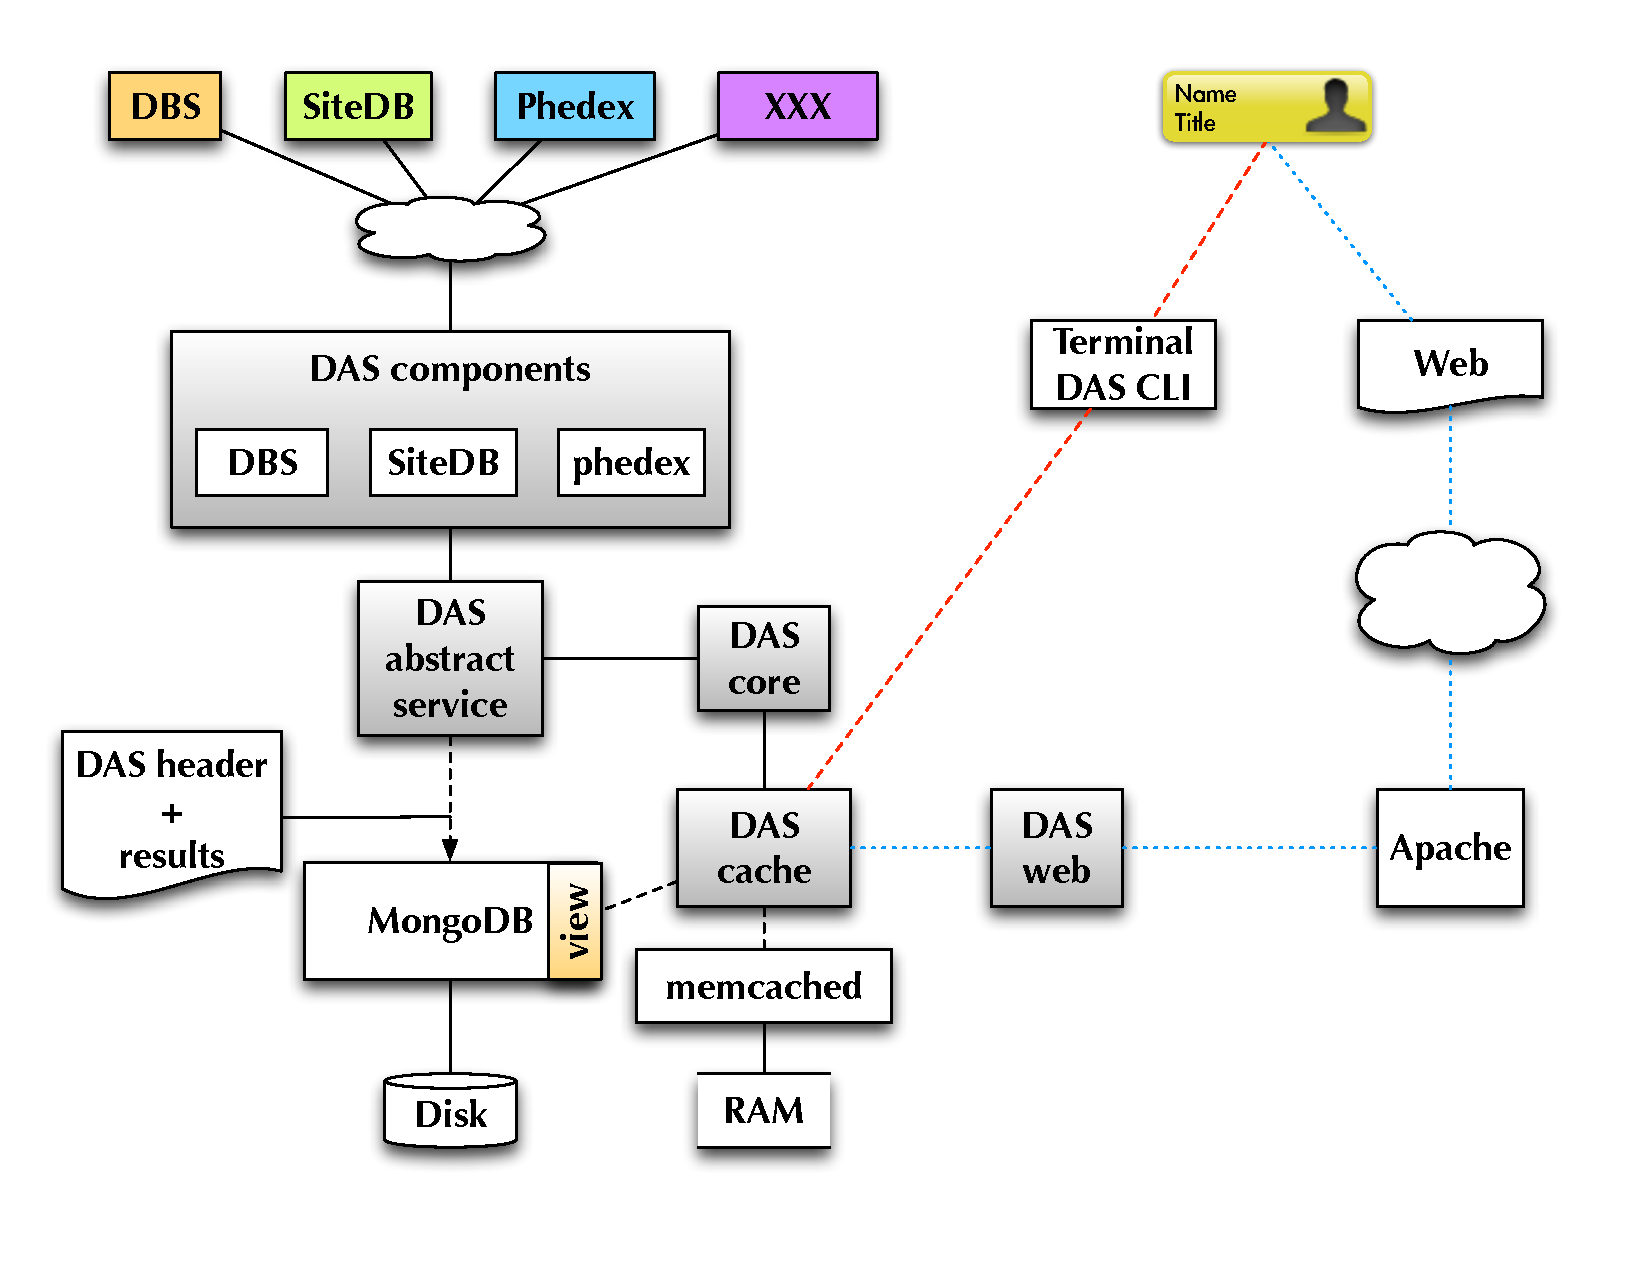
\includegraphics[width=150mm]{DAS_architecture.pdf}
\caption{
DAS architecture.
}
\label{DAS_arch}
\end{figure}

\begin{itemize}
\item DAS core system which is support pluggable modules to retrieve data from
CMS data-services, e.g. Data Bookkeeping System (DBS), data location service (Phedex),
etc.;
\item DAS caching system which has dual purpose: to store ``raw'' results coming
out from data-services, a raw-cache, and aggregated results produced by DAS core into
hot-cache;
\item DAS request service who collect and place into queue user requests
\item DAS mapping DB to store mapping between data-services and DAS notations and
data-representation;
\item DAS analytics DB to collect query statistics and establish pre-fetching 
strategies.
\end{itemize}
We will discuss each of those components in more details in up-coming sub-sections.
The DAS supports a pluggable approach to add a new CMS sub-system into a game by
identifying appropriate APIs, input and output parameters and keys, data-service
format and mapping between data-service, DAS and other sub-system. For instance,
the Data Bookkeeping System (DBS) and data location system (Phedex) store information about
a file. In former case, a file name was stored as well as its relations to other physics 
objects, such as run and luminosity, while in later case the Phedex store information 
about file location. When user specify a file as their selection key, based on
information store in DAS mapping DB we were able to identify appropriate set of
data-service APIs, look-up data, re-format their output to DAS notations and
store it into DAS raw-cache. Even though we support a data retrieval on demand
basis we also store user queries into DAS analytics DB to identify
a common patterns. Based on this information we organized a pre-fetching
populators. Once data were coming to raw-cache an additional step of
aggregation was applied. If other data with identical keys were presented in
a raw-cache we merge it them together. For instance upon the following query
$find file where ... $ a file information from DBS and Phedex systems were
retrieved. Since both data-services output contained file name as a common
key, their output where merged and final result was stored into raw-cache.
This merged (aggregated) results were shipped back to client and stored into
hot-cache (memcached) to speed up a DAS web client application. Each DAS data
object contains a standard DAS header, which identify look-up time,
request url, API, parameters and method as well as response version, expiration
time and checksum of the output. 

\subsection{DAS Query Language}
Upon success of DBS-QL \ref{DBS-QL} we adopted its syntax to DAS with a few minor
changes. Here we briefly recall its syntax:
\begin{equation}
action\,\,\,
key_1,\, key_2,\, ...\,\,\, where\,\,\,
\langle key\rangle\, 
\langle op\rangle\, 
\langle value\rangle \,\,\, and|or ...
\label{QL_syntax}
\end{equation}
Each DAS QL expression starts with special keyword indicating an action such as 
$find,\, plot,\, summary$, followed by a set of selection keys. The action identify
the behavior of the query, find to look-up data, plot to plot found data, summary to
apply a summary view over provided selection keys. An optional conditions can be 
specified via $where$ keyword following by condition expression.
Each condition expression represented via $key\,\,\, operator\,\,\, value$ triplet, where
$key$ is DAS selection key, $operator$ is conditional operator, 
$=,\, >=,\, <,\, in,\, between$ and $value$ is a value applied to selection key.
We also support brackets as well as $and$ and $or$ logical operators.
The DAS selection and condition keys were identified based on analysis 
of terminology used by our users. For instance, $file$ was used to either
select file name or used in condition to identify file name provided by user.
Here is a simple example of DAS QL expression:
$$
find\,\,\, file,\, run\,\,\, where\,\,\, site=T1\_CH\_CERN
$$
which represents a natural language question: 
{\it find files and runs located at T1\_CH\_CERN site}.

\subsection{DAS Mapping DB}
As been discussed above we used a DAS mapping DB to map data-service API into
DAS as well as map provide a relations between different data-services.
Upon identification of APIs which participate in DAS activity 
we store a mapping between data-service notations
into DAS mapping DB. This allows to map user input query parameters into
data-service API metrics as well as map back data-service output into DAS names.
For instance, the DBS system used $logical\_file\_name$ notation, while in Phedex
the same entity was named as $lfn$. Since both of them were referred to
logical file name, we map both notations into $file$ notation in DAS.\footnote{We
also deal with physical file names, but still used $file$ to refer to them in
DAS notation, since simple regular expressions were used to identify $file$
meaning from the provided value.}
For each service we provide a mapping from its own data-format (JSON, XML, etc.) into
common data-format used in DAS.\footnote{We used JSON as a DAS data format}
We also store a mapping between DAS keywords and data-service API names to
establish appropriate calls to data-service upon provided DAS query. For example,
when user specifies $file$ in their DAS query, we invoke DBS listFiles and Phedex
fileReplicas APIs. Since all mapping kept in RDMS we were able to abstract the 
DAS core library calls from hardcoded data-service API calls and make it
transparent to any participating data-services. Here is a logic of DAS core
library:
\begin{itemize}
\item parse input DAS query
\item map provided selection and condition keys into data-service APIs and
input parameters
\item invoke data-service APIs
\item parse output results by mapping output notation into DAS keys
\item store and aggregate them into DAS raw-cache
\end{itemize} 

\subsection{DAS Analytics DB}

\subsection{Caching system}
The DAS caching system was divided into two different caches: raw-cache and hot-cache.
The purpose of raw-cache was to store results coming from data services for
as long as specified in data-service response header. While the purpose of hot-cache
was to keep final DAS results corresponding to provided user query. We use a populator
services (jobs) to feed raw-cache with highly requested queries. Here we will only
discuss the raw-cache organization. 
\begin{figure}[htb]
\centering
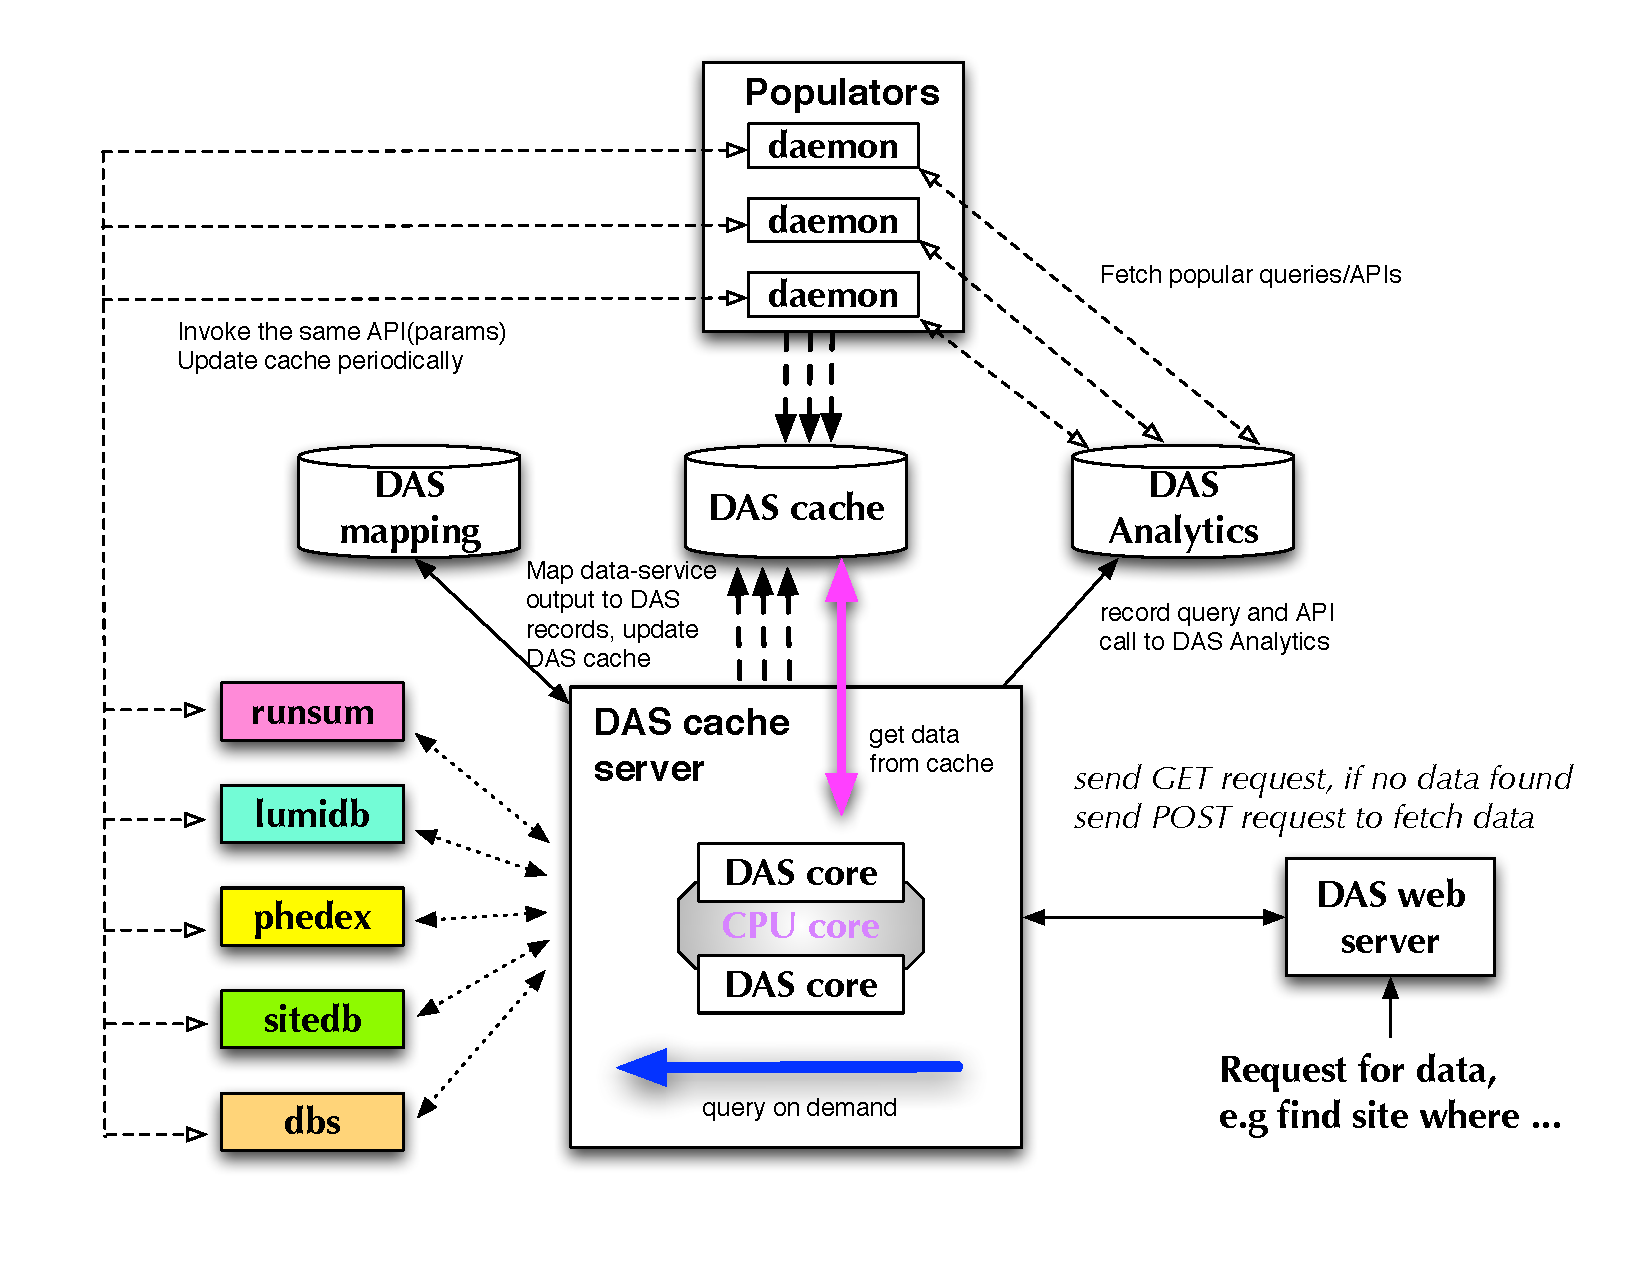
\includegraphics[width=150mm]{DAS_Cache_and_Analytics.pdf}
\caption{
DAS cache system.
}
\label{DAS_cache}
\end{figure}
As it shown in figure \ref{DAS_cache} the DAS cache server has dual purpose.
On one side it talks to DAS Analytics DB to trigger jobs for worker robot
who update cache with most popular queries, on another it talks to DAS
raw-cache back-end to either stored mapped results or merge them with 
existing DAS objects in a cache. We should note that we use on-demand
approach to answer user queries, but at the same time with a help of
DAS Analytics DB we force worker robots (populators) to pre-fetch
the most popular queries up-front.

We evaluated several technologies
as a choice for DAS cache back-end, including relational MySQL DB \cite{MySQL} 
and object oriented CouchDB \cite{CouchDB} and MongoDB \cite{MongoDB}.
Each of them had its own pros and cons. For instance usage
of MySQL provided a SQL queries (as in federated DBs, see \cite{FedDB}), but
required auto-schema generation on a fly.\footnote{We did not apply any
restriction to DAS QL and did not know in advance what our users will be
querying.} While, using CouchDB and MongoDB, we were able to store
data-service output naturally as documents objects into DB. Finally we decided
to use MongoDB due to its flexible and
powerful querying syntax, which were easy to map into DAS QL expressions. 

\subsection{REST interface}
We designed DAS interface to be fully REST complaint \cite{REST}.
All requests placed into DAS cache server were done via GET/PUT/POST/DELETE methods.
DAS clients initiate their request via GET method. An appropriate message
with either resulting data or their absense was send back to client.
Clients were able to decided upon received message how to proceed, either
request data via POST/PUT methods, DELETE data in cache or initiate another
GET request. The REST complaince help us to treat our clients, user quyering
DAS system via web browser, other CMS applications and command line tools
in identical manner. Also, the implementation of pre-fetch populator
tools become as easy and identical as any other clients.

\section{Results\label{Results}}

\section{Summary}

\section{Acknowledgements}

This work was supported by the National Science Foundation and Department of Energy of the United States of America. Fermilab is operated by Fermi Research Alliance, LLC under Contract
No. DE-AC02-07CH11359 with the United States Department of Energy.

\section*{References}
\begin{thebibliography}{9}
\bibitem{DBS} A. Afaq, et. al. ``The CMS Dataset Bookkeeping Service'', CHEP 2007 
\bibitem{DBS07} A. Dolgert, V. Kuznetsov, C. Jones, D. Riley, 
``A multi-dimensional view on information retrieval of CMS data'', CHEP 2007
\bibitem{DBS-QL} V. Kuznetsov, D. Riley, A. Afaq, V. Sekhri, Y. Guo, L. Lueking,
``The CMS DBS Query Language'', CHEP 2009
\bibitem{DD} https://cmsweb.cern.ch/dbs\_discovery

\bibitem{Arms}
C. R. Arms, W. Y. Arms, ``Mixed Content and Mixed Metadata 
Information Discovery in a Messy World'',
chapter from ``Metadata in Practice'', ALA Editions, 2004
\bibitem{DBXplorer}
Sanjay Agrawal, Surajit Chaudhuri, Gautam Das: DBXplorer: A System for
Keyword-Based Search over Relational Databases. ICDE 2002: 5-16

\bibitem{QueryAnswer}
Georgia Koutrika, Alkis Simitsis, Yannis E. Ioannidis: Pr\'{e}cis: The Essence of
a Query Answer. ICDE 2006: 69-78

\bibitem{FedDB}
L. Haas, E. Lin,
``IBM Federated Database Technology'', \\
http://www.ibm.com/developerworks/data/library/techarticle/0203haas/0203haas.html

\bibitem{MySQL}
http://www.mysql.com/

\bibitem{CouchDB}
http://couchdb.apache.org/

\bibitem{MongoDB}
http://www.mongodb.org/

\bibitem{REST}
Fielding, Roy Thomas ``Architectural Styles and the Design of 
Network-based Software Architectures'', Doctoral dissertation, 2000,
University of California, Irvine

\end{thebibliography}

\end{document}


